\section{Anomaliedaten}
\label{sec:data_anomalie}
Für Anomaliedaten werden die bekannten Routen modifiziert, indem Umleitungen eingebaut werden, die teilweise Standorte überspringen
und nicht in den Trainingsdaten vorhanden sind.
Dadurch wird ein Szenario simuliert, in der das Klassifizierungsverhalten vom ML-Modell zur Standortbestimmung auf unbekannten Wegen beobachtet werden kann.
Aus den Klassifizierungsergebnissen des ML-Modells zur Standortbestimmung werden schließlich Features extrahiert,
die vom ML-Modell zur Anomalieerkennung verwendet werden.
\begin{figure}[h!]
    \centering
    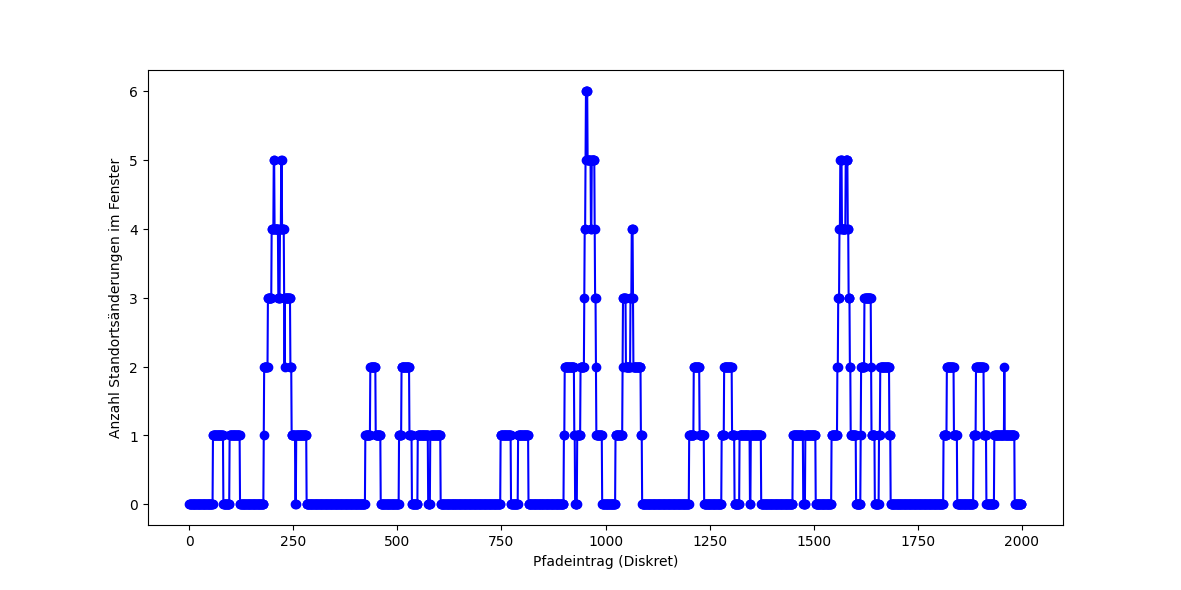
\includegraphics[width=\linewidth]{images/feature_window_location_changes.png}
    \caption{Ausschnitt der Anomalietestmenge mit den Standortänderungen in einem Datenfenster von 25.}
    \label{fig:window_location_changes}
\end{figure}
\newpage
Wenn eine Anomalie vorliegt, wird erwartet, dass das ML-Modell unsicherer wird und stärker fluktuiert,
wodurch drei Features motiviert sind.
Das erste Feature ist abgeleitet aus der Anzahl der Standortänderungen.
Das Feature ist der Betrag der Differenz von den folgenden Komponenten.
Die erste Komponente ist die durchschnittliche Anzahl der Standortänderungen in einem Datenfenster.
Die zweite Komponente die durchschnittliche Anzahl der Standortänderungen, wenn keine Anomalie vorliegt.
Abbildung \ref{fig:window_location_changes} zeigt die akkumulierten Standortänderungen in einem Datenfenster von 25.
Bei den Pfadeinträgen bei ca. 250, 1000 und 1600 sind Extrema zu erkennen, die mit der Anomalie in dieser Testmenge übereinstimmen,
d. h. wenn eine Anomalie vorliegt wird häufiger der Standort geändert.
\newline
\newline
Das zweite Feature ist analog zum ersten Feature konstruiert.
Dieses nutzt anstatt der Anzahl der Standortänderungen die summierte Wahrscheinlichkeit der erkannten Standorte.
Das ML-Modell zur Standortbestimmung hat keine diskrete Ausgabe, sondern gibt einen Vektor von Wahrscheinlichkeiten aus,
der für jeden Standort die Klassifizierungswahrscheinlichkeit angibt.
Dabei gilt der klassifizierte Standort als der Eintrag im Vektor mit der höchsten Wahrscheinlichkeit.
Diese Wahrscheinlichkeit wird dann analog zu den Standortänderungen summiert.
Das dritte Feature ist die Standardabweichung der ersten fünf Einträge dieses Vektors, der absteigend sortiert ist.
Abbildung \ref{fig:window_confidence} zeigt die akkumulierte Standortwahrscheinlichkeit in einem Datenfenster von 25.
Bei den Pfadeinträgen bei ca. 250, 1000 und 1600 ist die akkumulierte Standortwahrscheinlichkeit deutlich geringer als läge keine Anomalie vor,
d.~h. wenn eine Anomalie vorliegt, ist die Sicherheit für einen Standort geringer.
\begin{figure}[h!]
    \centering
    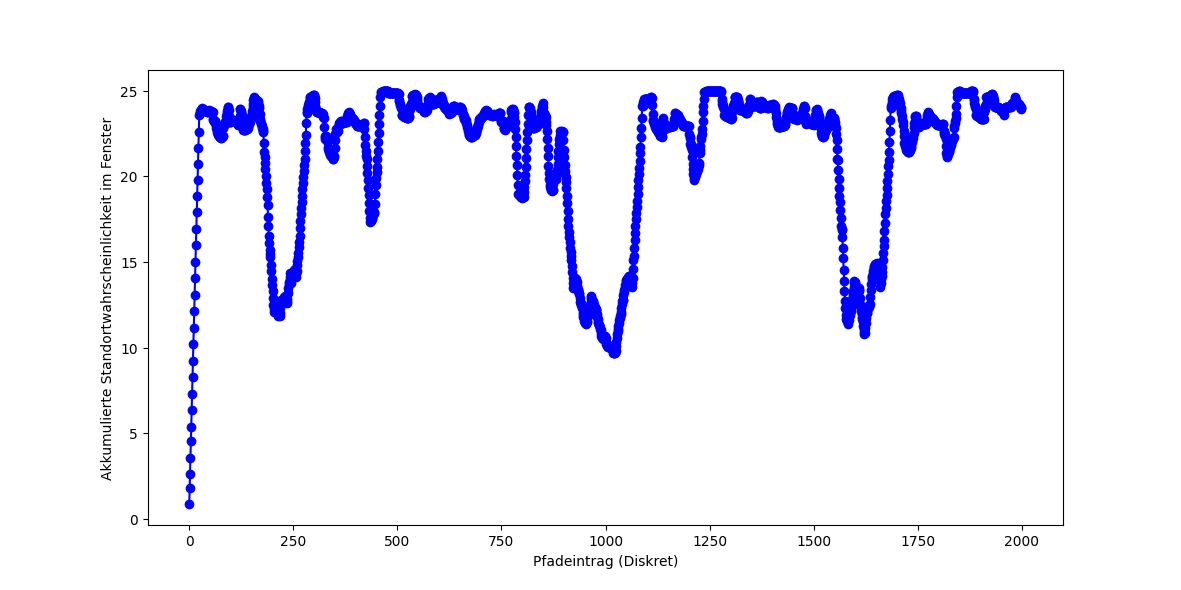
\includegraphics[width=\linewidth]{images/feature_window_confidence.png}
    \caption{Ausschnitt der Anomalietestmenge mit der akkumulierten Standortwahrscheinlichkeit in einem Datenfenster von 25.}
    \label{fig:window_confidence}
\end{figure}
\newline
\newline
Zusätzlich wird das Ergebnis des Modells auf Basis der Topologie als Feature verwendet.
Dieses Feature indiziert, dass das ML-Modell zur Standortbestimmung ein Fehler gemacht haben muss
oder dass tatsächlich eine Anomalie vorliegt, da die Topologie verletzt wurde.
\newline
\newline
Daneben wurde ebenfalls eine Rückwärtskante in Betracht gezogen,
da es wahrscheinlich ist, dass wenn zuvor eine Anomalie vorlag, danach immer noch eine Anomalie vorliegt.
Im Training wurden damit zwar sehr gute Ergebnisse erreicht,
in der Praxis war das Modell aber äquivalent zum \textit{Immer-Falsch} Modell.
